%\subsection{A First Use-Case:  Comparison of Entropy, Snooze and DVMS}
\subsubsection{Analysis of Entropy, Snooze and DVMS}
\label{subsec:first-usecase}
%\AL{Il faudra parler du nombre de migrations qui est egalement une
%  métrique pertinente. Plusieurs algorithms tentent de reduire cette
%  metrique }
%\AL[AL]{Il faudra mettre des snapshots de PajeNG}
% Evaluation of VMPlaceS on Grid'5000: simulations were running on one server.
In this paragraph, we discuss the results of the simulations we
performed on the Entropy,  Snooze and DVMS strategies.
% Due to space limitations we present a generaly study
% analyzing the violation times as well as the
% duration of the computation and reconfiguration phases. However, we
% highlight that such a study enables us to investigate some variant and possible
% improvements of Snooze and DVMS that made possible to easily study  thanks to
% \vmps.

%\subsubsection{Experimental Conditions}
Regarding the experimental conditions, all simulations have been
performed on the Lyon clusters of the Grid'5000 testbed.
Each execution was running on a dedicated server, thus avoiding
interferences between simulations and ensuring reproducibility between
the different invocations.
% Scripts: automation of the deployment, running of simulations and the collect
% of results.
% It enables us to run a large number of simulations, with several variants
% of the scheduling algorithm.
%
\vmps has been configured to simulate an homogeneous
infrastructure of PMs composed of 8 cores, 32~GB of RAM and 1~Gpbs
Ethernet NIC. To enable fair comparison between the three strategies,
the scheduling resolver only considered 7 cores (\ie one was devoted
to run the Snooze LC or the DVMS processes). Dedicating one core for
the host OS and other administrative processes is something which is
rather usual and thus we believe acceptable in our experimental
methodology.  Ten VMs have been
initially launched on each simulated PM. Each VM relied one of the VM
classes described in the accuracy experiment and the
parameters for changing the load were the same ($\lambda$ = Nb
VMs/300, $\mu$ = 60 and $\sigma$ = 20). The stationary state was
reached after 20 min of the simulated time with a global cluster load
of 85\%.
%as depicted in Fig. \ref{fig:load_figure}.
To accelerate the simulations, we have chosen to limit the simulated time to 1800
seconds. It is noteworthy that the consolidation ratio, \ie the number
of VMs per node, has been defined to generate a sufficient number of
violations. We discovered that under a global load of 75\%, our
infrastructure almost did not face VM violations with our selected Gaussian
distribution. Such a result is rather
satisfactory as it can explained why most production DCs target such
an overall utilization rate.\footnote{\url{http://www.cloudscaling.com/blog/cloud-computing/amazons-ec2-generating-220m-annually/}}
Finally, infrastructures composed of
128, 256, 512 and 1024 PMs, hosting respectively 1280, 2560, 5120 and
10240 VMs have been investigated. For Entropy and Snooze that rely on
service nodes, additional simulated PMs have been provided. For Snooze, one GM
has been created every 32 LCs (\ie PMs). The frequency to invoke the
solver has been setted to 30 seconds for Entropy and the Snooze GMs.
We remind that no service
node had to be provisioned for DVMS as a DVMS process has been
executed directly on top of each hosting node.
%
% In order to cope with real DC conditions, we defined the parameters
% for node crashes to simulate a fault on average every 6 months for a
% duration of 300 seconds. These values correspond to the Mean Time To
% Failure (MTTF) and the Mean Time To Repair (MTTR) of a Google DC
% server~\cite[pp. 107-108]{datacenterAsComputer}. We underline that at
% the scale we performed our simulations such a crash ratio was not
% sufficient to impact the behavior of the scheduling policies.
% Dedicated simulations were mandatory to study the influence of node
% crashes. However, due to the space limitations, we do not present them
% in the article and only gives major trends. Regarding Entropy,
% although the lost of the service node can be critic, the failure
% probability is so small that the single point of failure issue can be
% easily solved by a fail-over approach. Regarding Snooze, the heartbeat
% strategy enables the reconstruction of the hierarchy in a relative
% short time and thus crashes on service nodes do not significantly
% impact the resolution of violations (in our case less than 10 seconds
% is mandatory to reorganize the Snooze topology with a 6 seconds
% heartbeat mechanism). Finally regarding DVMS, the crash of one node
% does not have any impact of the resolution has the composition of the
% microcosm is reevaluated immediately.
%%
%Finally, we highlight that all configuration files used to perform the discussed simulations can
%be downloaded from the \vmps repository.

%\subsubsection{General  Analysis}
%\label{subsec:general-comparison}

% \begin{figure}
% \subcapcentertrue
% \subfigure[Infrastructure load]{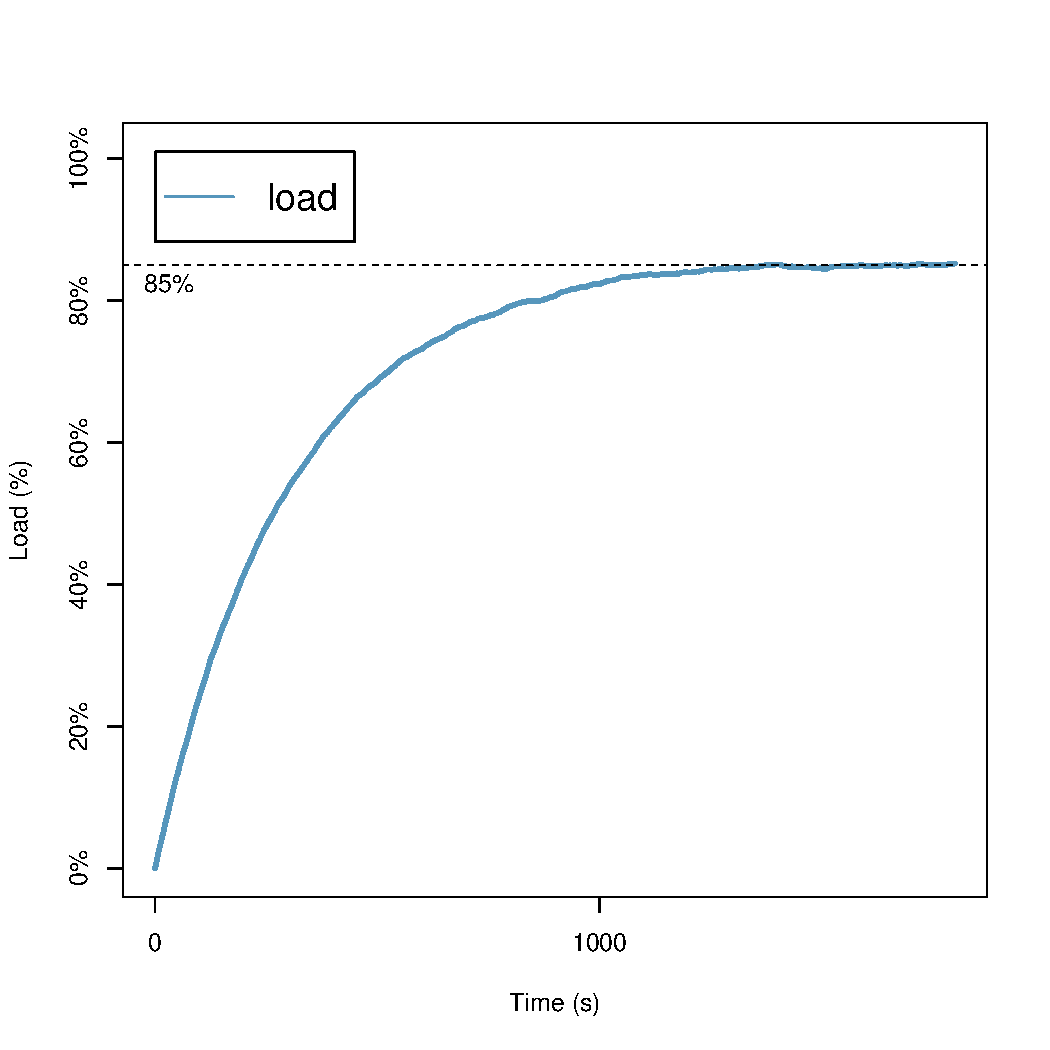
\includegraphics[width=4cm]{./figures/experiments/1024-hierarchical.pdf}\label{fig:load_figure}}
% \subfigure[Cumulated Violation Time]{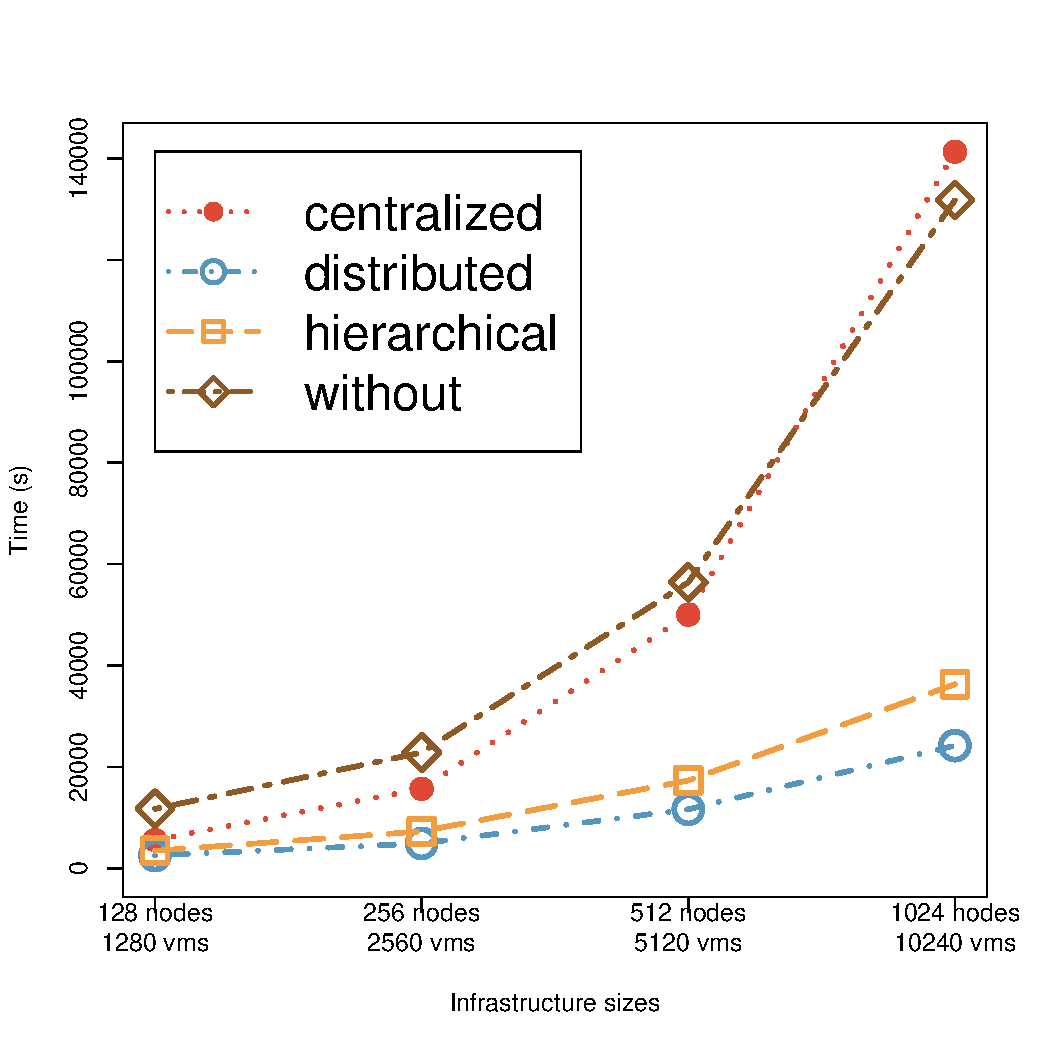
\includegraphics[width=4cm]{./figures/experiments/violation_time.pdf}\label{fig:cumulated_violation}}
% \caption{Simulation Results - 10 VMs per node (VM load: $\mu=60$ and $\sigma=20$)}
% \label{fig:simulation-overview}
% \end{figure}

\begin{figure*}
\subcapcentertrue
\subfigure{
  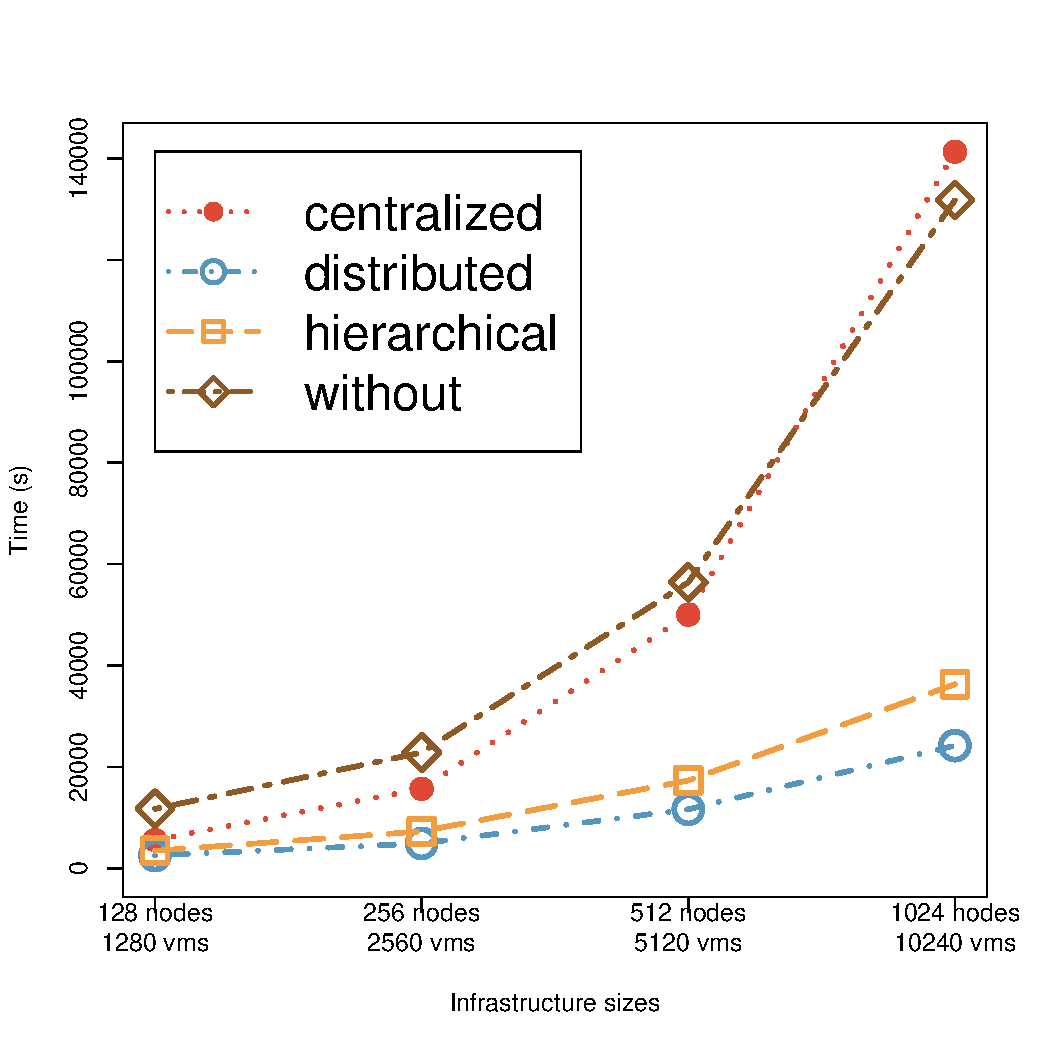
\includegraphics[width=.46\textwidth]{figures/experiments/violation_time.pdf}
  \label{fig:violationTime}}
\begin{minipage}{.5\textwidth}
\centering
  \vspace*{-6cm}
%\subfigure[Duration of violation ($med \pm \sigma$)]{
\subfigure{
    {\tiny \begin{tabular}{|P{17mm}@{\:}||@{\:}c@{\:}|@{\:}c@{\:}|@{\:}c@{\:}|}
      \thickhline
      \textbf{Infrastructure size}
        & \multicolumn{3}{c@{\:}|}{\textbf{Duration of violations}
          ($med \pm \sigma$)}
          \Tstrut \\
         \hfill  & ~Centralized~ & ~Hierarchical~ & Distributed \Bstrut \\
      \thickhline
         128 nodes & 23.19 $\pm$ 14.17  & 10.82 $\pm$ 4.66  & 9.89 $\pm$ 2.97 \\
         256 nodes & 40.32 $\pm$ 25.67  & 10.93 $\pm$ 4.72  & 9.52 $\pm$ 2.56 \\
         512 nodes & 57.39 $\pm$ 44.17  & 11.43 $\pm$ 7.12  & 9.64 $\pm$ 2.89 \\
        1024 nodes & 79.15 $\pm$ 82.39  & 12.02 $\pm$ 9.53  & 9.68 $\pm$ 2.73
        \Rstrut  \\ \hline
      \thickhline
  \end{tabular} }
%\label{table:detailed_violation_time}
}
  \vspace*{-.2cm}

%\subfigure[Duration of computations ($Med \pm \sigma$)]{
\subfigure{
    {\tiny \begin{tabular}{|P{17mm}@{\:}||@{\:}c@{\:}|@{\:}c@{\:}|@{\:}c@{\:}|}
      \thickhline
      \textbf{Infrastructure size}
        & \multicolumn{3}{c@{\:}|}{\textbf{Duration of computations}
          ($med \pm \sigma$)}
          \Tstrut \\
         \hfill  & ~Centralized~ & ~Hierarchical~ & Distributed \Bstrut \\
      \thickhline
         128 nodes  &  6.75 $\pm$  9.23  & 10.56 $\pm$ 1.35  & 0.02 $\pm$ 0.02 \\
         256 nodes  & 14.71 $\pm$ 19.11  & 10.57 $\pm$ 1.19  & 0.02 $\pm$ 0.01 \\
         512 nodes  & 27.67 $\pm$ 35.61  & 10.53 $\pm$ 1.27  & 0.02 $\pm$ 0.01 \\
        1024 nodes  & 37.80 $\pm$ 63.14  & 10.61 $\pm$ 1.63  & 0.02 $\pm$ 0.02 
      \Rstrut  \\ \hline
      \thickhline
  \end{tabular} }
%\label{table:detailed_computation_time}
}
  \vspace*{-.2cm}

%\subfigure[Duration of reconfigurations ($Med \pm \sigma$)]{
\subfigure{
    {\tiny \begin{tabular}{|P{17mm}@{\:}||@{\:}c@{\:}|@{\:}c@{\:}|@{\:}c@{\:}|}
      \thickhline
      \textbf{Infrastructure size}
        & \multicolumn{3}{c@{\:}|}{\textbf{Duration of  reconfigurations}
          ($med \pm \sigma$)}
          \Tstrut \\
         \hfill  & ~Centralized~ & ~Hierarchical~ & Distributed \Bstrut \\
      \thickhline
         128 nodes & 10.08 $\pm$ 0.84 & 10.07 $\pm$ 0.77 & 10.06 $\pm$ 0.76 \\
         256 nodes & 10.82 $\pm$ 2.60 & 10.05 $\pm$ 0.64 & 10.05 $\pm$ 0.65 \\
         512 nodes & 13.86 $\pm$ 4.83 & 10.07 $\pm$ 0.75 & 10.05 $\pm$ 0.65 \\
        1024 nodes & 23.24 $\pm$ 6.53 & 10.18 $\pm$ 1.09 & 10.08 $\pm$ 0.73 
      \Rstrut  \\ \hline
      \thickhline
  \end{tabular} }
%\label{tab:detailed_reconf_time}
}
\end{minipage}
\vspace*{-.6cm}
\caption{Scalability/Reactivity analysis of Entropy, Snooze and DVMS}
\label{fig:general-comparison}
\vspace*{-.8cm}
\end{figure*}

Fig.~\ref{fig:general-comparison} presents on the left the cumulated violation
time for each placement policy and on the right several tables that give more details by presenting the
mean and the standard deviations of the duration of, respectively, the
violations and the computation/reconfiguration phases. As
anticipated, the centralized approach did not scale and became almost
counterproductive for the largest scenario in comparison to a system
that did not use any dynamic scheduling strategy. The more nodes Entropy has to
monitor, the less efficient it is on both the computation and
reconfiguration phases. Regarding the computation, the VMPP is a
NP-Hard problem and thus it is not surprising that it takes more time
to resolve larger problems. Regarding the reconfiguration, as Entropy
has to solve much more violations simultaneously, the reconfiguration plan
is more complex for large scenarios, including several migrations
coming from and going to the same nodes. Such reconfiguration plans
are non optimal as they increase the bottleneck effects at the network
level of each involved PM. Such a simulated result is valuable as it confirms
that reconfiguration plans should avoid as much as possible such
manipulations.
%
Regarding Snooze, although the performances are better than the
Entropy ones, we may erroneously conclude that the hierarchical
approach is not competitive with respect to the distribued strategy at
the first sight. However, diving into details, we can see that both
the computation and reconfiguration phases are almost constants
(around 3 seconds and 10 seconds) and not so far from the DVMS values,
especially for the reconfiguration phase, which is predominant. These
results can be easily explained: the centralized policy adresses the
VMPP by considering all nodes at each invovation, while the
hierarchical and the distributed algorithms divide the VMPP into sub
problems, considering smaller numbers of nodes (32~PMs in Snooze and
4 in average with DVMS). To clarify the influence of the group size on
the Snooze performances, \ie the ratio of LCs attached to one GM, we
performed additional simulations aiming at investigating whether a
smaller group size can lead to similar performances of DVMS. We
higlight that the use of \vmps eased such a study as it has consisted
to simply relaunch the previous simulation with a distinct
assignment.


\begin{figure*}
  \vspace*{-.5cm}
\subcapcentertrue
%\subfigure[Total Violation Times]{
\subfigure{
  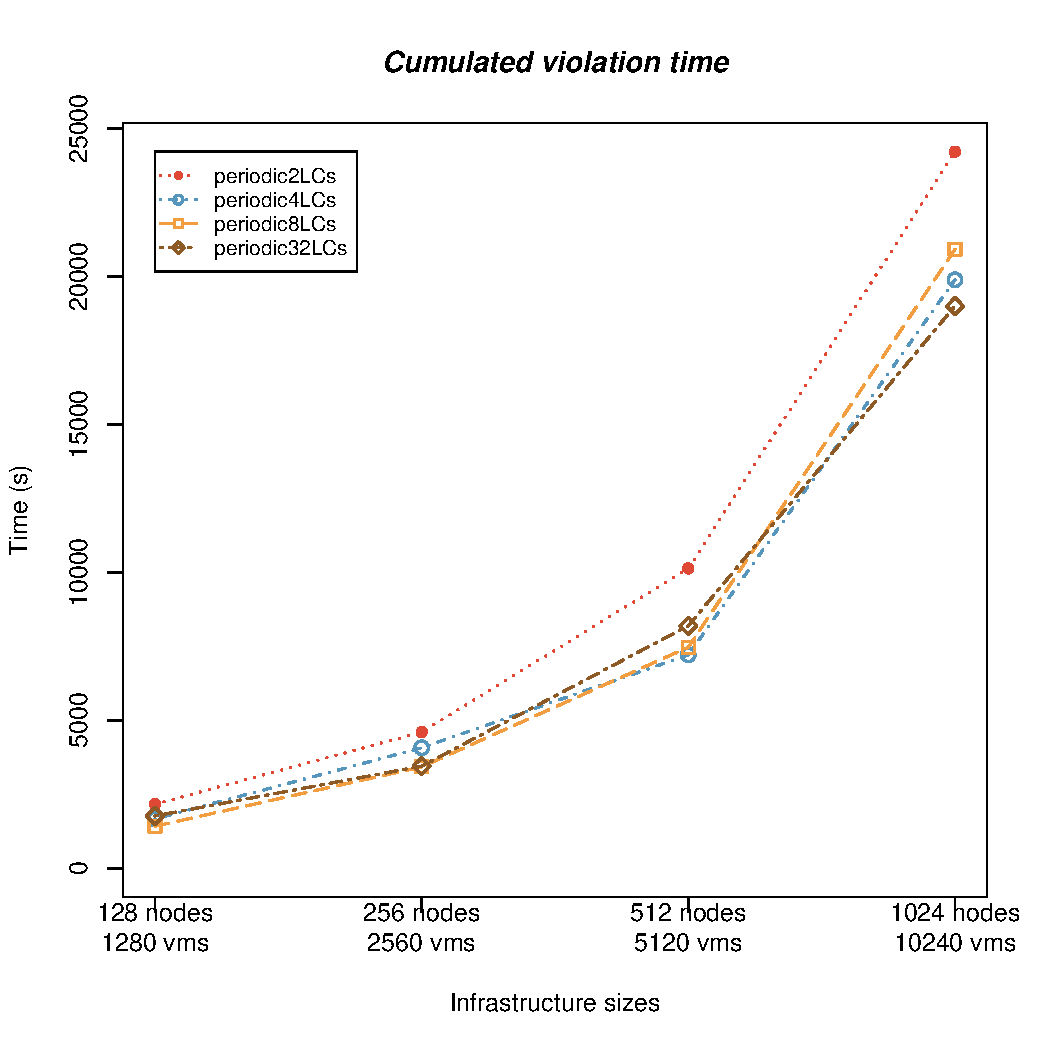
\includegraphics[width=.38\textwidth]{figures/groupSizes-violationTime.pdf}
  \label{fig:groupSizesViolationTime}}
\begin{minipage}{.60\textwidth}\centering
  \vspace*{-4.5cm}
%\subfigure[No.\ of Failed Reconfigurations]{
\subfigure{
    {\tiny \begin{tabular}[b]{|r@{\:}||@{\:}r@{\:}|@{\:}r@{\:}|@{\:}r@{\:}|@{\:}r@{\:}|}
      \thickhline
      \textbf{Infra.\ Size~~}
        & \multicolumn{ 4 }{c@{\:}|}{\textbf{No.\ of failed reconfigurations}}
          \Tstrut \\
         \hfill &  ~2 LCs~ & ~4 LCs~ & ~8 LCs~ &  ~32 LCs~  \Bstrut \\
      \thickhline

        128~~~~~~~ &  19~ & 0~ & 0~ & 0~ \\
        256~~~~~~~ &  29~ & 0~ & 0~ & 0~ \\
        512~~~~~~~ &  83~ & 1~ & 0~ & 0~ \\
       1024~~~~~~~ & 173~ & 7~ & 0~ &  0
      \Rstrut  \\ \hline
      \thickhline
  \end{tabular} }
  \label{fig:groupSizesReconfigFail}
  }
\vspace*{-.2cm}

%\subfigure[Means $\pm$ Std deviations of computation durations.]{
\subfigure{
    {\tiny \begin{tabular}[b]{|r@{\:}||@{\:}c@{\:}|@{\:}c@{\:}|@{\:}c@{\:}|@{\:}c@{\:}|}
      \thickhline
      \textbf{Infra.\ Size~~}
        & \multicolumn{ 4 }{c@{\:}|}{\textbf{Duration of the
            computations $(Med \pm \sigma)$}}
          \Tstrut \\
         \hfill &  ~2 LCs~ & ~4 LCs~ & ~8 LCs~ & 32 LCs  \Bstrut \\
      \thickhline

        128~~~~~~~ &   0.16 $\pm$   1.23 &   0.34 $\pm$   1.81 &   0.58 $\pm$   2.40 &   2.53 $\pm$   4.62  \\
        256~~~~~~~ &   0.18 $\pm$   1.31 &   0.42 $\pm$   1.99 &   0.66 $\pm$   2.50 &   2.65 $\pm$   4.69  \\
        512~~~~~~~ &   0.15 $\pm$   1.20 &   0.33 $\pm$   1.78 &   0.67 $\pm$   2.54 &   2.83 $\pm$   4.98  \\
       1024~~~~~~~ &   0.19 $\pm$   1.37 &   0.42 $\pm$   2.02 &   0.89 $\pm$   2.90 &   ~2.69 $\pm$   4.91

      \Rstrut  \\ \hline
      \thickhline
  \end{tabular} }
  \label{fig:groupSizesComputationTime}
  }
\end{minipage}
\vspace*{-.6cm}
\caption{Hierarchical placement: influence of varying group sizes}
\label{fig:snoozeGroupSizes}
\vspace*{-.6cm}
\end{figure*}
%
%\paragraph{Varying group sizes}
%
Figure \ref{fig:snoozeGroupSizes} presents the simulated values
obtained for scenarios with 2,~4,~8 and 32~LCs per GM for four
infrastructure sizes. The overall performance (\ie cumulated violation
time) shows that
2~LCs per GM result in significantly higher violation times.
% All other
%group sizes yield violation times that are relatively close, which
%indicates that a small group size does not help much in
%resolving violations faster.
The relatively bad performance of the smallest group size can be
explained in terms of the number of failures of the reconfiguration
process, that is, overloading situations that are discovered but
cannot be resolved because the GM managing the overloaded VM(s) did
not dispose of enough resources (see tables on the right).
Groups of 2~LCs per GM are clearly insufficient at our global load level (85\%).
Failed reconfigurations are, however, already very rare in the case of
4~LCs per GM and do not occur at all for 8~and 32~LCs per GM. This is
understandable because the load is statistically evenly distributed
among the LCs and tthe load profile we evaluated only rarely results
in many LCs of a GM to be overloaded. Violations can therefore be
resolved even in the case of a smaller number (4) LCs available for
load distribution.
Conversely, we can see that the duration of the computation phases
decreases strongly along with the group
size. It reaches a value close to the computation times of DVMS for a
group size of 4-LCs per GM.% see Fig.~\ref{fig:groupSizesComputationTime}.
We thus cannot minimize computation times and violation times by
reducing the number of LCs because larger group sizes are necessary to
resolve overload situations if the VM load gets higher.
In contrast, DVMS resolves this trade-off by construction because of its
automatic and dynamic choice of the partition size necessary to handle
an overload situation.
Once again,
this information is valuable as it will help researchers to design new
algorithms favoring the automatic discovery of the optimal subset of
nodes capable to solve violations under for given load profiles.

\vmps provides additional metrics such as the number of migrations
that has been performed overall, the average duration of each
migration~\ldots. Due to space limitations, we cannot discuss all
these metrics. However, we emphasize that they provide importance
guidances on the pros and cons of each scheduling policy, notably on
the migration overhead on the network but
also on the workload running inside each VM.

Moreover,  we underline that we succeeded to conduct DVMS simulations including
up to 8K~PMs/80K~VMs in a bit less than two days. We did not present
such results to the paper because it was not possible to run a
sufficient number of Snooze simulations at such scale. The Snooze
protocol being more complex than the DVMS one (heartbeats,
consensus,~\ldots), the time to perform a similar experiment is much
more important (around 7 days). The time-consuming portions of the
code are related to \sg internals such as \texttt{sleep} and
\texttt{send/recv} calls. Hence, we have contacted the \sg core
developers in order to investigate how we can reduce the required time
to perform such advanced simulations.

Last but not the least, the study performed in this paper has
highlighted several variants and possible improvements such as a
reactive approach of Snooze instead of a periodical one, a more
aggresive partitionning integration for DVMS~\ldots. All these
variants can be easily studied and evaluated thanks to VMPlaceS.
